\chapter{Methodology}
\label{ch:methodology}

This thesis is conducted within the Design Science Research (DSR) paradigm, in which the construction and evaluation of an artifact is the central research contribution \cite{hevner2004designscience, peffers2007dsrm}; Sec.~\ref{sec:research-approach} develops this orientation.
The process by which that artifact was produced is organised using the Double Diamond model \cite{designcouncil2023diamond}, a human-centred design framework introduced by the Design Council that structures a design project into two sequential diverge-then-converge cycles.
The first diamond covers the problem space: an initial phase of wide exploration that opens up the inquiry, followed by a focusing phase that narrows the findings into a precise, actionable problem statement.
The second diamond covers the solution space: a generative phase that develops and iterates on the solution, followed by a delivery phase that converges on a tested, evaluated artifact (in this thesis, delivering the artifact and evaluating it against the research questions).
Fig.~\ref{fig:double-diamond} illustrates this structure and maps each phase to the corresponding stage of this thesis.

\begin{figure}[htbp]
\centering
\resizebox{0.92\linewidth}{!}{%
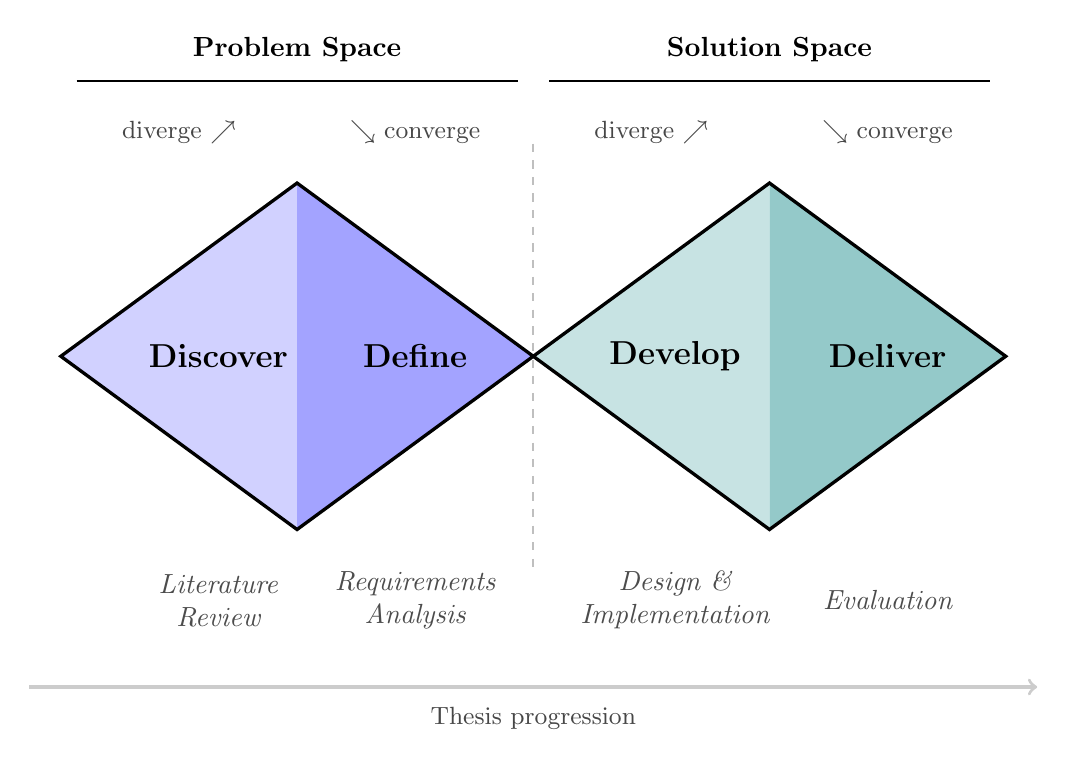
\begin{tikzpicture}[
  phlbl/.style={font=\large\bfseries, align=center},
  thlbl/.style={font=\normalsize\itshape, align=center, text=gray!60!black},
  spanlbl/.style={font=\normalsize\bfseries, align=center},
  dirlbl/.style={font=\small, align=center, text=gray!55!black},
]

%% ── Colours ──────────────────────────────────────────────────────────────────
\colorlet{discoverFill}{blue!18}
\colorlet{defineFill}{blue!36}
\colorlet{developFill}{teal!22}
\colorlet{deliverFill}{teal!42}

%% ── Diamond 1 — Problem Space (x: 0 → 6, apex at 3) ─────────────────────────
\fill[discoverFill] (0,0) -- (3, 2.2) -- (3,-2.2) -- cycle;
\fill[defineFill]   (3,2.2) -- (6,0)  -- (3,-2.2) -- cycle;
\draw[very thick]   (0,0) -- (3,2.2) -- (6,0) -- (3,-2.2) -- cycle;

%% ── Diamond 2 — Solution Space (x: 6 → 12, apex at 9) ───────────────────────
\fill[developFill]  (6,0) -- (9, 2.2) -- (9,-2.2) -- cycle;
\fill[deliverFill]  (9,2.2) -- (12,0) -- (9,-2.2) -- cycle;
\draw[very thick]   (6,0) -- (9,2.2) -- (12,0) -- (9,-2.2) -- cycle;

%% ── Vertical divider between diamonds ────────────────────────────────────────
\draw[dashed, thick, gray!50] (6, 2.7) -- (6,-2.7);

%% ── Phase name labels (inside each quadrant) ─────────────────────────────────
\node[phlbl] at (2.0,  0) {Discover};
\node[phlbl] at (4.5,  0) {Define};
\node[phlbl] at (7.8,  0) {Develop};
\node[phlbl] at (10.5, 0) {Deliver};

%% ── Thesis-phase labels (below each quadrant) ────────────────────────────────
\node[thlbl] at (2.0, -3.1) {Literature\\Review};
\node[thlbl] at (4.5, -3.1) {Requirements\\Analysis};
\node[thlbl] at (7.8, -3.1) {Design \&\\Implementation};
\node[thlbl] at (10.5,-3.1) {Evaluation};

%% ── Diverge / Converge annotations ──────────────────────────────────────────
\node[dirlbl] at (1.5,  2.85) {diverge $\nearrow$};
\node[dirlbl] at (4.5,  2.85) {$\searrow$ converge};
\node[dirlbl] at (7.5,  2.85) {diverge $\nearrow$};
\node[dirlbl] at (10.5, 2.85) {$\searrow$ converge};

%% ── Problem / Solution space span labels ─────────────────────────────────────
\draw[thick] (0.2, 3.5) -- (5.8, 3.5);
\node[spanlbl] at (3.0, 3.9) {Problem Space};

\draw[thick] (6.2, 3.5) -- (11.8, 3.5);
\node[spanlbl] at (9.0, 3.9) {Solution Space};

%% ── Overall flow arrow (below thesis-phase labels) ───────────────────────────
\draw[->, very thick, gray!40] (-0.4, -4.2) -- (12.4, -4.2);
\node[font=\small, text=gray!55!black] at (6.0, -4.6) {Thesis progression};

\end{tikzpicture}%
}
\caption[The Double Diamond process model as applied in this thesis.]{%
The Double Diamond process model \cite{designcouncil2023diamond} as applied in this thesis.
Each diamond represents one diverge-then-converge cycle:
the first covers the problem space (literature review and requirements analysis)
and the second covers the solution space (design and implementation, then evaluation).
Italic labels below each phase name indicate the corresponding thesis activity.%
}
\label{fig:double-diamond}
\end{figure}

The remaining sections of this chapter detail each methodological dimension in turn.
Sec.~\ref{sec:research-approach} describes the research approach that guides the four phases.
Sec.~\ref{sec:requirements-elicitation} explains how requirements were derived.
Sec.~\ref{sec:development-process} describes the iterative engineering process and tooling.
Sec.~\ref{sec:evaluation-strategy} sets out the evaluation strategy.
Sec.~\ref{sec:tools-and-technologies} describes the development tooling and the use of generative-AI assistance.
Sec.~\ref{sec:ethical-considerations} addresses ethical considerations arising from the use of eye-tracking data.

\section{Research Approach}
\label{sec:research-approach}

This thesis is a platform engineering thesis: its primary contribution is a designed and implemented software artifact (a researcher-operated adaptive reading platform) rather than an empirical study of human reading behaviour.
The research approach is therefore shaped by the nature of that contribution: the goal is not to measure a natural phenomenon but to construct, justify, and evaluate a designed system.
The Double Diamond model \cite{designcouncil2023diamond}, introduced at the opening of this chapter, serves as the overarching process framework, organising the work into two sequential diverge-then-converge cycles that cover the problem space and the solution space respectively.

This artifact orientation determines what counts as a research output in this thesis.
Design decisions are first-class contributions that must be motivated, documented, and evaluated, not merely implemented.
The architecture itself (the separation of sensing, decision-making, intervention execution, and researcher interface into independently replaceable modules) is the central claim this thesis makes, and the evaluation is designed to assess whether that claim holds in the implemented system.

The research questions stated in \cref{sec:final-problem-statement} reflect this orientation directly.
RQ1 through RQ4 all ask about properties of the designed system (modularity, sensing pipeline feasibility, context-preserving intervention, and researcher experimentability), not properties of human reading behaviour.
This is a deliberate boundary: whether specific typographic interventions measurably improve reading outcomes for participants is a question for a future empirical study conducted with this platform, and it is explicitly outside the scope of this work.
The platform is the instrument that makes such future studies possible; building and validating that instrument is the contribution of this thesis.

\section{Requirements Elicitation}
\label{sec:requirements-elicitation}

Requirements for this platform were derived through retrospective analysis of an existing prototype rather than up-front specification.
Because a prototype of the adaptive reading system already existed at the start of this thesis work, we began by analysing that prototype alongside the original project proposal \cite{ref1} and the findings of the literature review to identify what a research-capable platform must be able to do.
This analysis produced an initial set of requirements that was then refined through regular supervision sessions, during which gaps and implicit assumptions in the prototype were surfaced and made explicit.

User stories were written from the perspective of the three primary actors (the researcher, the participant, and the external module provider) and were used as the primary vehicle for communicating behavioural expectations across the team.
Functional and non-functional requirements were then derived from those user stories, with the non-functional requirements specifically motivated by the architectural goals of the thesis: modularity, low latency, extensibility, and reproducibility.
Each requirement was assigned a MoSCoW priority (Must have, Should have, Could have, or Won't have) \cite{clegg1994moscow}, providing a principled basis for identifying the minimum viable capability set and for deferring lower-priority features when time pressure required trade-offs.

We note that this elicitation approach is a deliberate consequence of the thesis type.
Because the contribution is an artifact, the requirements serve a dual purpose: they establish what the system must do, and they provide the criteria against which the architectural design decisions in \cref{ch:design} are later justified.

\section{Development Process}
\label{sec:development-process}

The system was developed by a team of two as an iterative build, with each iteration targeting a coherent vertical slice of functionality (from sensing to decision to intervention to researcher interface) rather than building one layer at a time.
This approach was chosen over a design-first waterfall process for two reasons.
First, the integration between the Tobii hardware layer, the realtime transport, and the frontend intervention rendering could not be fully specified upfront: latency, timing, and synchronisation constraints only become visible under end-to-end execution.
Second, a vertical-slice structure ensures that integration assumptions are tested and corrected at each increment rather than deferred to a final integration phase, reducing the risk of late-stage architectural surprises.
This iteration takes place within the Develop phase of the second diamond: the Double Diamond describes the overall diverge-then-converge progression of the thesis, not a single linear pass through implementation, which instead advanced as repeated build-test-correct increments.

The codebase is organised as a monorepo containing five sub-projects: the frontend application, the backend API and realtime server, the documentation site, a reference decision-maker, and a reference eye-movement analyser.
This structure allowed shared conventions and contracts to be maintained across components without requiring a separate package registry, while keeping each sub-project independently buildable and deployable.

Version control was managed using Git with GitHub as the remote host.
Changes were introduced through pull requests, providing a lightweight code-review step between the two authors before merging to the main branch.
The CI pipeline configuration is described in \cref{sec:tools-and-technologies}.

The full codebase is published on GitHub and released under the MIT License, making it freely available for inspection, reuse, and extension by future researchers and developers.
This decision reflects the open-science orientation of the work: because the architecture and the integration contracts are themselves research contributions, making the source openly accessible is necessary for those contributions to be reproducible and verifiable by others.

\section{Evaluation Strategy}
\label{sec:evaluation-strategy}

The evaluation of this thesis addresses three distinct questions that together cover the four research questions of \cref{sec:final-problem-statement}: whether the system functions correctly as a platform for reading experiments, whether the architecture satisfies the modularity and extensibility goals that motivate the design, and whether its runtime behaviour meets the live-operation constraints that adaptive reading imposes.
Tab.~\ref{tab:rq-evaluation} maps each research question to the method by which it is evaluated, and the remainder of this section describes those methods.

\begin{table}[htbp]
\centering
\caption{Mapping of each research question to its evaluation method. The reading-behaviour effect study that a full evaluation of intervention efficacy would require is outside the scope of this thesis.}
\label{tab:rq-evaluation}
\begin{tabular}{p{0.30\linewidth} p{0.60\linewidth}}
\toprule
Research question & Evaluation method \\
\midrule
RQ1 --- Modularity & Dependency-graph inspection (no imports across module boundaries), module-installer review, and demonstration that a reference provider connects without modifying the core. \\
RQ2 --- Sensing pipeline & Measurement of end-to-end gaze-to-event and gaze-to-intervention latency under live operation, and confirmation that the analysis stage is inspectable, loggable, and replayable. \\
RQ3 --- Context-preserving intervention & Demonstration that interventions are committed at controlled boundaries, together with inspection of the logged context-preservation events. \\
RQ4 --- Researcher control & Demonstration of the researcher's session controls and verification of the auditable record through session replay and data export. \\
\bottomrule
\end{tabular}
\end{table}

For functional correctness, we evaluate the system against the functional requirements defined in \cref{ch:requirements}, verifying that each requirement is met through a combination of automated tests, manual end-to-end walkthroughs of the researcher and participant workflows, and inspection of exported session data.
For architectural quality, we evaluate the degree to which the modular boundaries between sensing, decision-making, intervention execution, and user interface hold in the implemented system, and whether the external module provider integration contract is sufficient for a third-party provider to connect without modifying the core application.
Concretely, the architectural-quality assessment summarised in the RQ1 row of Tab.~\ref{tab:rq-evaluation} is carried out through three means:
\begin{enumerate}
  \item Inspection of the dependency graph to confirm that no module imports across the boundaries defined in the design.
  \item Demonstration that the external integration contract is sufficient for the reference decision-maker sub-project to connect to the core runtime without modifying it.
  \item Review of the module installer pattern to confirm that new implementations can be substituted at the composition root without touching application logic.
\end{enumerate}

The remaining methods in Tab.~\ref{tab:rq-evaluation} concern the runtime behaviour of the platform rather than its structure: the gaze-to-event and gaze-to-intervention latency measurement for RQ2, and the boundary-commit and session-replay demonstrations for RQ3 and RQ4, are carried out as part of the evaluation reported in \cref{ch:evaluation}.

We acknowledge one structural threat to validity: as a two-person implementation team, we cannot assess our own architectural decisions with full objectivity.
We partially mitigate this, by enabling external scrutiny: we publish the codebase and integration contracts openly under the MIT License, making them available for independent inspection, and we treat the reference decision-maker and reference eye-movement analyser as independently exercised validators of the external integration contract rather than as internal tests.

We do not conduct a user study of reading behaviour within the scope of this thesis.
The platform is designed to enable such studies, but evaluating the effectiveness of specific typographic interventions on reading comprehension or fatigue is a separate research question that requires a dedicated experiment with recruited participants and an approved study protocol.
That question is explicitly outside the scope of this work, as discussed in \cref{ch:introduction}.

\section{Development Tooling and AI Assistance}
\label{sec:tools-and-technologies}

The rationale for the platform's technology stack is architectural rather than methodological, and is therefore presented with the other design decisions in \cref{sec:technology-selection}.
This section records two aspects of how the artifact was produced: the tooling that kept it continuously validated during development, and the use of generative-AI assistants.

Throughout development the codebase was kept continuously buildable and testable through two independent continuous-integration pipelines, one for each sub-project, so that every change was validated automatically.
The engineering practices behind this, including the automated test suite and the Windows build environment required by the eye-tracking hardware (C1), are detailed in \cref{ch:implementation}.

In keeping with contemporary software practice, generative-AI assistants were used in a limited, supporting role during the project.
Their use was bounded to three tasks: coding assistance for the software artifact, feedback and rephrasing on prose the authors had already written, and a sounding board for discussing design trade-offs the authors had already formed.
All AI-assisted output was reviewed, verified, and (where it was code) tested by the authors, who remain responsible for the result; the analysis, the design decisions, and the prose of this thesis are the authors' own.
A full declaration of generative-AI use, including the specific tools and the tasks for which they were used, is provided in \cref{app:ai-declaration}.

\section{Ethical Considerations}
\label{sec:ethical-considerations}

Eye-tracking data is sensitive by nature: it captures where a person directs their attention, moment by moment, and can in principle be used to infer cognitive states, reading difficulties, or other personal characteristics beyond the scope of any individual experiment.
Collecting such data from study participants therefore requires careful handling.

Within this platform, all session data (including raw gaze samples, demographic attributes, and comprehension results) remains under the direct control of the researcher who operates the system.
No data is transmitted to external servers; all storage is local to the machine on which the backend is running.
Participant attributes collected at enrolment (name, age, sex, existing eye conditions, and reading proficiency) are stored only within the session record and are not shared outside the system.

Because these attributes are directly identifiable, researchers deploying the platform in a real study should apply pseudonymisation where required by their study protocol, replacing identifying fields with participant codes before any data leaves the controlled research environment.
Data should be retained only for the duration required by the study protocol and applicable regulations, and deleted thereafter.

The development of this platform did not itself require an institutional ethics review, as no human participants were recruited and no personal data was collected during the engineering work described in this thesis.

The ethics obligations described above apply to researchers who deploy the platform in a future study involving real participants.
Before conducting such a study, the researcher is responsible for obtaining informed consent from each participant, ensuring that participants understand what data is collected and how it will be used, and complying with applicable data protection regulations, including the General Data Protection Regulation (GDPR) \cite{gdpr2016} as it applies at DTU.
The platform does not implement consent workflows directly; this responsibility rests with the researcher conducting the study.

\section*{Chapter Summary}

This chapter established the methodological foundations of the thesis.
The Double Diamond model was introduced as the overarching process framework, mapping the four phases of the research (literature review, requirements analysis, design and implementation, and evaluation) onto two sequential diverge-then-converge cycles covering the problem space and the solution space respectively.
The research approach was characterised as artifact-oriented, treating the constructed artifact and its architectural decisions as primary research outputs.
The engineering process was described as iterative and vertical-slice driven, with continuous integration, pull-request-based review, and open-source publication supporting reproducibility and extensibility.
Requirements were shown to be derived through retrospective analysis of an existing prototype, refined through supervision sessions, and expressed as user stories and MoSCoW-prioritised requirements.
The evaluation strategy was defined around two questions: functional correctness verified against the requirements, and architectural quality assessed through dependency inspection and external contract validation; a structural threat to validity was acknowledged and mitigated through open publication of the codebase.
Ethical responsibilities arising from the collection of gaze and participant data were identified and assigned to the researcher operating the platform.
The requirements derived through the process described here are presented in full in the following chapter.

